\chapter{Results}

This chapter presents the findings of the experiments conducted in this masters thesis. The chapter is divided into two sections.
The first section presents the results of\method{1}, the second section presents the results of \method{2}, where both methods will be evaluated in context of both Gaussian VAEs and VQ-VAEs. In the final section, I will present the cross-validation results of the both methods.

\section{Results of \method{1}}

In this section, I will present the results of \method{1} on both Gaussian VAEs and VQ-VAEs.

\subsection{Results on Gaussian VAEs}

The experiments showed similar results for both exact sampling and uniform sampling. The results showed that \method{1} can be used not only to obtain a condiotioned decoder, but also to improve the quality of non-conditioned decoder reconstruction when compared to non-conditioned Gaussian VAEs. However, KL divergence loss of the latent space increased when \method{1} was applied. This can be explained by the fact that the there is a trade-off between the quality of the reconstruction and the KL divergence of the latent space. An example of this can be seen in the figure  \ref{fig:res_val} and \ref{fig:results_method1_gaussian_vae}. 

When comparing the results of the exact same sampling and uniform sampling it showed little difference to each other.

In order to exclude and verify that I the results are not due to the architecture of the neural network, I applied range of loss balancing techinques such as coefficient balancing and applying SoftAdapt. After applying these techinques it could still be observed that the quality of the reconstruction was improved in expense of a slightly higher KL divergence loss of the latent space.

When trying to use deeper neural networks on the Gaussian VAEs, I observed that the posterior collapse was more likely to happen, which is a common problem in Gaussian VAEs~\cite{wang2023posterior}.
% Think about: Coefficients, Number of pixels to be sampled. How it changes the results.

\begin{figure}[H]
    \centering
    \centering
\scriptsize
\begin{tabular}{||c|c|c|c||}
\hline
 Method & Parameters & Reconstruction loss & KL loss \\
\hline
\textit{Baseline} & - & 0.0042 +- 1.2e-03 & 0.0018 +- 6.3e-04 \\
\hline
Multi Decoder & Exact sampling & 0.0036 +- 8.3e-04  $\downarrow$ & 0.0027 +- 8.7e-04  $\uparrow$ \\
\hline
Multi Decoder & Exact sampling, SoftAdapt & 0.0034 +- 1.9e-04  $\downarrow$ & 0.0029 +- 2.8e-03  $\uparrow$ \\
\hline
Multi Decoder & Uniform sampling & 0.0035 +- 6.5e-04  $\downarrow$ & 0.0026 +- 1.7e-03  $\uparrow$ \\
\hline
Multi Decoder & Uniform sampling, SoftAdapt & 0.0034 +- 7.3e-03  $\downarrow$ & 0.0029 +- 2.0e-02  $\uparrow$ \\
\hline
\end{tabular}

    \caption[Trained neural network with \method{1} applied to a Gaussian VAE.]
    { 
        Trained neural network with \method{1} with Exact same sampling applied to a Gaussian VAE on CelebA dataset and latent space 16. 
        On the left side as input is the original image, on the right side there are two outputs of the decoders. 
        The image from the condiotioned decoder is reconstructed with a higher quality compared to the non-conditioned decoder, because the condiotioned decoder $Decoder_2$ uses conditioning information $m$.
    }
    \label{fig:res_val}
\end{figure}


\begin{figure}[H]
    \centering
    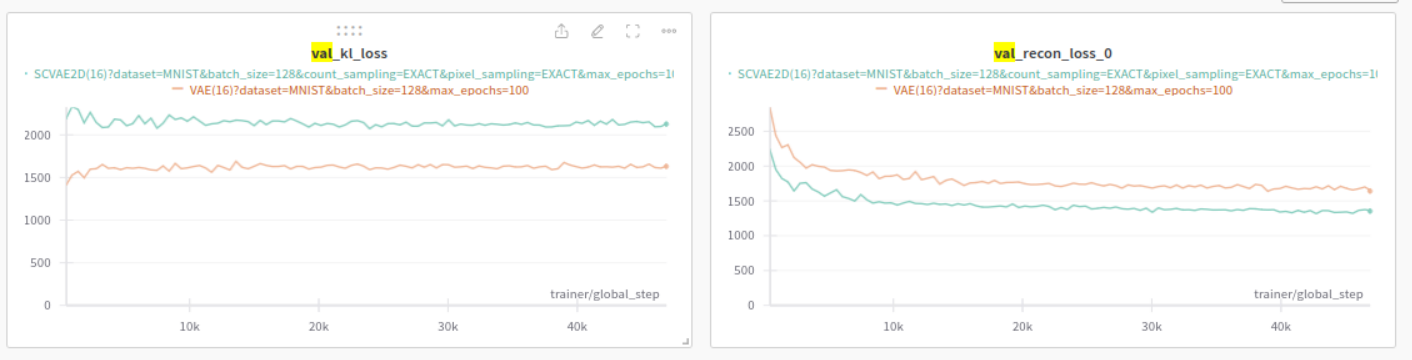
\includegraphics[width=0.8\textwidth]{figures/results/KL_and_RECON.png}
    \caption[Validation loss comparison during training of a Gaussian VAE.]
    {
        Validation loss comparison with and without \method{1} applied during training of a Gaussian VAE.
        Left: KL divergence loss of the latent space comparison. Right: Reconstruction loss comparison of the $Decoder_1$ - non conditioned decoder.
    }
    \label{fig:results_method1_gaussian_vae}
\end{figure}

\subsection{Results on VQ-VAEs}

When applying \method{1} to VQ-VAEs, the results showed that both the quality of the reconstruction and the VQ objective loss improved, which could be observed for both exact same sampling and uniform sampling. This could be explained by the fact that the VQ-VAEs are more robust and stable compared to Gaussian VAEs.

Same as previously mentioned the method was applied with SoftAdapt loss balaning technique and without it. Th results showed little to no difference between the two. However, the training stability was improved when using SoftAdapt with less fluctuaiions in the loss.



\subsubsection{Exact same sampling}

\subsubsection{Uniform sampling}


\section{Results of \method{2}}

In this section, I will present the results of \method{2} on both Gaussian VAEs and VQ-VAEs.

\subsection{Results on Gaussian VAEs}

\subsubsection{Uniform random sampling}


\subsubsection{Gaussian sampling}

\subsection{Results on VQ-VAEs}

\subsubsection{Uniform random sampling}

\subsubsection{Gaussian sampling}


